\documentclass{article}
\usepackage[utf8]{inputenc}

\title{SRS - Searching for and navigating to a location}
\author{Nardus van der Vyver }
\date{February 2017}

\usepackage{natbib}
\usepackage{graphicx}
\usepackage[table,xcdraw]{xcolor}

\begin{document}

\maketitle

\begin{table}[]
\centering
\label{my-label}
\begin{tabular}{|l|l|}
\hline
\rowcolor[HTML]{EFEFEF} 
Use Case         & Searching for a location                                                                                                                                                                                                                                                                                                                                                                  \\ \hline
Description      & \begin{tabular}[c]{@{}l@{}}Type your location into the search bar in order \\ for the application to search for the \\ building/location.\end{tabular}                                                                                                                                                                                                                                    \\ \hline
Precondition     & \begin{tabular}[c]{@{}l@{}}It has to be a location inside the Hatfield \\ campus of The University of Pretoria.\end{tabular}                                                                                                                                                                                                                                                              \\ \hline
Assumption       & \begin{tabular}[c]{@{}l@{}}1. You are connected to TUKS Wi-Fi.\\ 2. You know the name of your destination\\ \\ building.\end{tabular}                                                                                                                                                                                                                                                     \\ \hline
Cases            & \begin{tabular}[c]{@{}l@{}}1. Click on the search bar and start typing\\ the \\ location you are interested in.\\ 2. If the location is not found make sure\\ \\ everything is spelled correctly.\\ 3. Choose your destination from a list of\\ \\ possible locations.\\ 4. Click on the directions link in order for the\\ \\ program to display the route to your location\end{tabular} \\ \hline
Expected results & \begin{tabular}[c]{@{}l@{}}1. After typing in the search bar the\\ location \\ you are interested in is displayed.\\ 2. You click on your destination.\\ 3. The application displays the directions from\\ \\ to point you are now to your destination.\end{tabular}                                                                                                                      \\ \hline
\end{tabular}
\end{table}

\begin{table}[]
\centering
\label{my-label}
\begin{tabular}{|l|l|}
\hline
\rowcolor[HTML]{EFEFEF} 
Use Case         & Navigating to chosen location                                                                                                                                                                                                                                                                                                                                                         \\ \hline
Description      & \begin{tabular}[c]{@{}l@{}}The application will guide you through campus \\ towards the destination of choice, making your \\ route the shortest possible with the least \\ amount of traffic.\end{tabular}                                                                                                                                                                           \\ \hline
Precondition     & \begin{tabular}[c]{@{}l@{}}1. You are connected to TUKS Wi-Fi and have a \\ stable connection.\\ 2. You already chose your destination by \\ searching for it.\end{tabular}                                                                                                                                                                                                           \\ \hline
Assumption       & \begin{tabular}[c]{@{}l@{}}1. You are connected to TUKS Wi-Fi with a \\ stable connection.\\ 2. You know where you want to go.\end{tabular}                                                                                                                                                                                                                                           \\ \hline
Cases            & \begin{tabular}[c]{@{}l@{}}1. The application shows you the route to follow.\\ 2. You lose your Wi-Fi connection and the \\ application has to wait or  recalculate your position.\\ 3. While walking the application recalculates your \\ route based on the  traffic ahead.\\ 4. While walking the app shows your present \\ location and whether  you arrived or not.\end{tabular} \\ \hline
Expected results & \begin{tabular}[c]{@{}l@{}}1. The application shows the shortest route with \\ least amount of traffic.\\ 2. As you walk you follow along to make sure you \\ are on track.\\ 3. The application will let you know when you arrive.\end{tabular}                                                                                                                                      \\ \hline
\end{tabular}
\end{table}

\begin{figure}
\centering
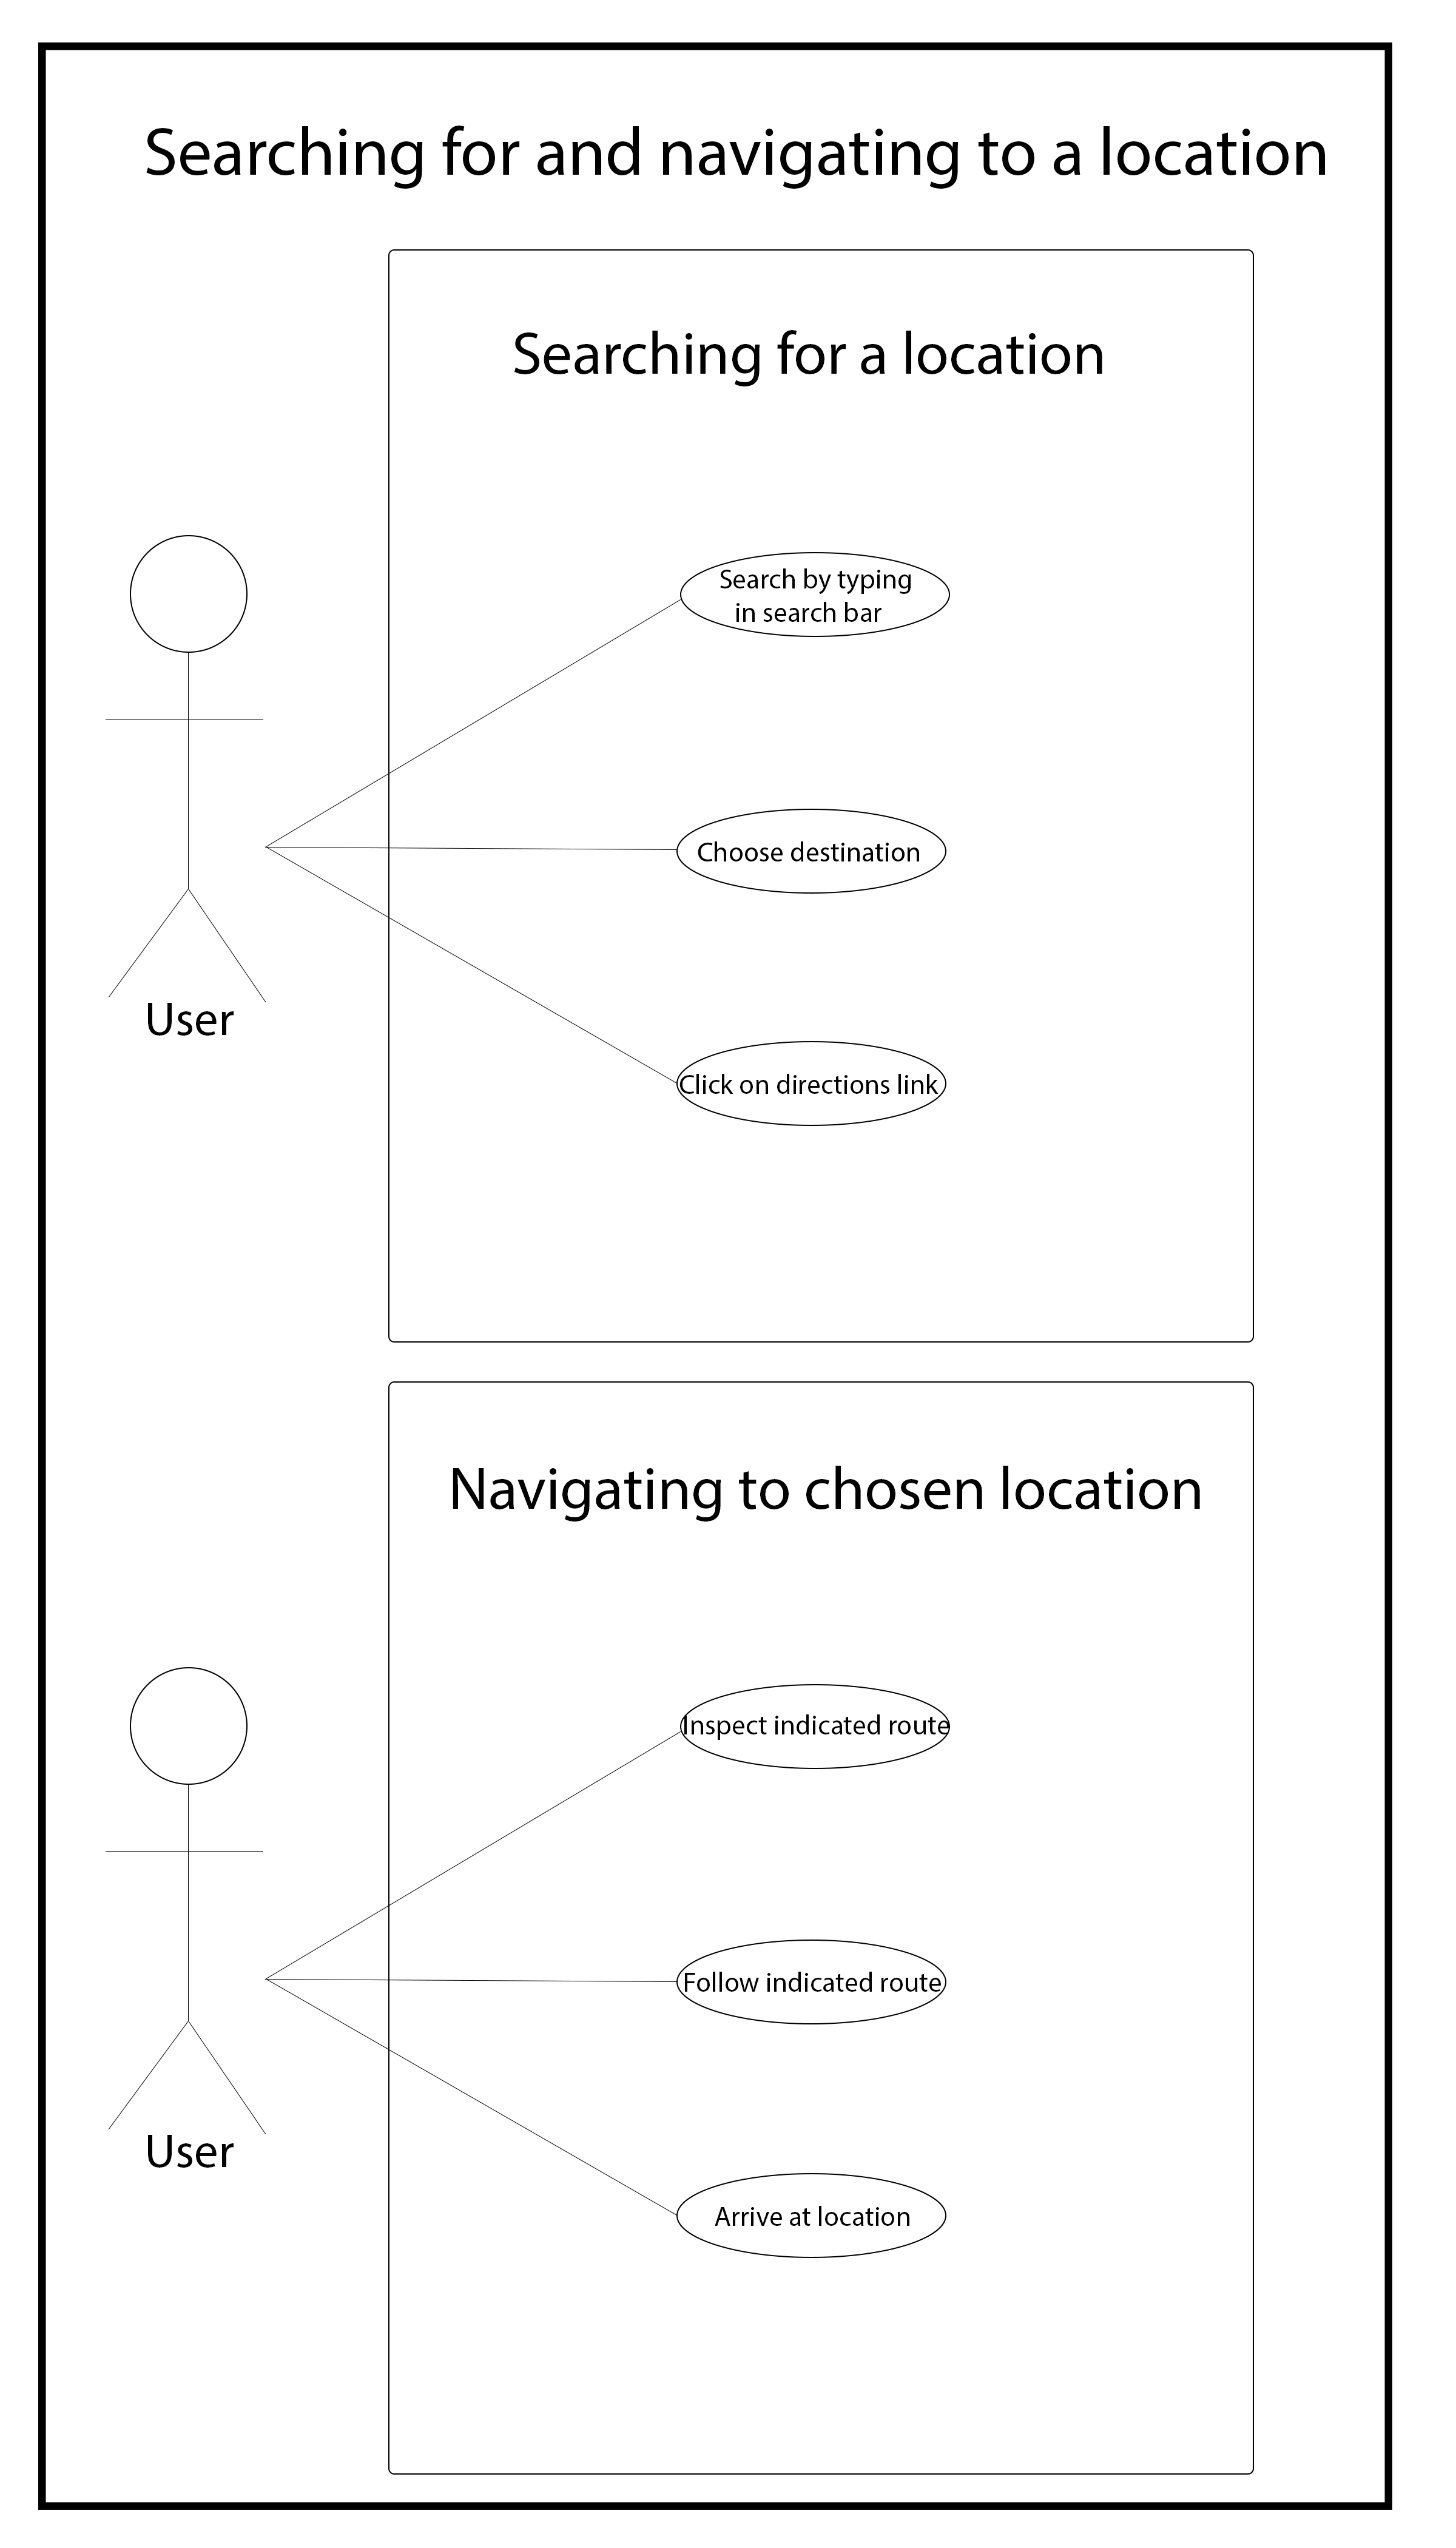
\includegraphics[scale=0.5]{SandN.png}
\caption{UML Diagram}
\label{UML diagram}
\end{figure}


\end{document}